\newpage
\appendix
\setcounter{equation}{0}      
\section{Convolutional Neural Network model (CNN)}\label{app:CNN}

\textbf{Preprocessing.}
We performed the following preprocessing steps on the dataset:
\begin{enumerate}
    \item Each frame was cropped on half of the image since the rest is
          completely out of the retina field of view (frame dimension: 864 →
          432
          pixels / 3024 → 1512 microns).
    \item It was downsampled by a factor of 4 (frame dimension: 432 → 108 pixels /
          3.5 → 14 microns per pixel)
    \item Each pixel value was standardized by subtracting the mean and
          dividing
          by the standard deviation of the pixel values of the whole dataset.
    \item Spikes during the presentation of the natural image was binned into
          16 bins of 25ms to produce a 16-bin PSTH for each mini-movie. Spikes
          during the
          adaptation images aren’t used at all.
    \item 80\% of the data was used for training, and 20\% for validation.
          Testing was done on a separate dataset.
\end{enumerate}

\textbf{Model architecture.}
The first layer of the CNN model was a convolutional layer with S
two-dimensional convolutional kernels, where the filters were learned from the
data.
The second layer was composed of a single three-dimensional filter and a vector
of feature weights (with one weight
for each of the features extracted by the first layer) followed by a
non-linearity.
Using a common filter for all the features helps reduce the number of
parameters, following previous work \citep{cadena_deep_2019}.

The model is composed of:
\begin{enumerate}
    \item Convolutional kernel weights $k_{rstk}$ that compute convolutions
          with
          the input images (where $r$ and $s$ index the single kernel spatial
          dimensions, $t$ indexes time,
          and $k$ indexes kernels).
    \item Pointwise nonlinear functions
          $f_{\theta_k^{[1]}}$ that convert the convolutional outputs
          into non-negative activation values.
    \item In addition, for each neuron $n$:
          \begin{enumerate}
              \item Readout weights $w_{ijtk}$ which can be factorized as
                    $w_{ijtk} =
                        u_{ijt}v_{kn}$, where $i$ and $j$ index space, $t$
                    indexes time, $u_{ij}$ represent the spatial
                    weights, and $v_{k}$ the feature weights.
              \item A pointwise nonlinear function
                    $f_{\theta^{[2]}}$.
          \end{enumerate}
\end{enumerate}

We choose $f_{\theta_k^{[1]}}$ to be ReLU functions ; \[
    \text{ReLU}(x) =
    \begin{cases}
        x, & \text{if } x \geq 0 \\
        0, & \text{if } x < 0
    \end{cases}
\].

$f_{\theta_n^{[2]}}$ was selected to be a softplus function :
$\text{softplus}(x) = \ln(1 + e^x)$. It was used as a smoothed ReLU.

In practice, we fix the nonlinearities in the implementation and learn their
threshold in the model as bias in the convolutional layer, which is strictly
equivalent to learning the threshold of the nonlinearities.

The outputs (activation map) of the $k$th unit of the first layer
were:
\[
    A_k = f_{\theta_k^{[1]}} (\sum_{k} K_k \cdot X) \
\]

The spiking rate $r$ of the neuron given an input image $X$ on the temporal bin
number $n$
was:
\[
    r_n(X) = f_{\theta_n^{[2]}} (\sum_{k} \sum_{ij,t \in [t_0 - 7, t_0]}
    u_{ijt}v_{kn}A_{ijtk})
\]

Additionally, batch normalization was applied to the outputs of the first
layer as well as between the filter and the feature weights of the second
layer.

Batch normalization normalizes the activations in a batch of data
during training. It is typically applied before the activation function.
The goal is to mitigate issues related to internal covariate
shifts and facilitate faster convergence.

In batch normalization, given a batch of inputs $X = \{x_1, x_2, \ldots,
    x_m\}$ for a layer, the following steps are performed:

1. Compute the mean and variance of the batch:
\[
    \mu = \frac{1}{m} \sum_{i=1}^{m} x_i \quad \text{and} \quad \sigma^2 =
    \frac{1}{m} \sum_{i=1}^{m} (x_i - \mu)^2
\]

2. Normalize the batch using the mean and variance:
\[
    \hat{x}_i = \frac{x_i - \mu}{\sqrt{\sigma^2 + \epsilon}}
\]

Where $\epsilon$ is a small constant added for numerical stability.

3. Scale and shift the normalized values with learnable parameters:
\[
    y_i = \gamma \hat{x}_i + \beta
\]

The parameters $\gamma$ and $\beta$ are learned during training through
backpropagation.

\textbf{ Regularization on Convolutional Kernels}

We employed a L2 regularization applied to the convolutional kernels of the
first layer:

\[
    L_{2^{[1]}} = \lambda_{2^{[1]}} \sum_{i,j,t} (\lvert k_{ijt} \rvert^2)
\]

Here, $K_{rsk}$ represents the convolutional kernels, $\epsilon = 10^{-8}$ is a
small constant, and $p$ sums over all the relevant indices.

The L1 and L2 regularizations applied to the spatial weights and feature
weights of the second layer are given by:

\[
    L_{1^{[2]}} = \lambda_{1^{[2]}} \sum_{i,j,t} \lvert u_{ijt} \rvert
\]

\[
    L_{2^{[2]}} = \lambda_{2^{[2]}} \sum_{i,j,t} (\lvert u_{ijt} \rvert^2)
\]

Here, $\lambda_{2^{[1]}} $, $\lambda_{1^{[2]}}$ and $\lambda_{2^{[2]}}$ are the
regularization hyperparameters,
and $k_{ijt}$, $u_{ijt}$ represent the spatiotemporal weights of the first and
second layer respectively.

\textbf{Model training.}
Considering the m recorded video-response pairs $(X1, y1).., (Xn,yn)$ the
resulting loss function is given by:
\[
    L= \frac{1}{m} \sum_{k=1}^{m} \frac{1}{n} \sum_{l=1}^{m} (r(X_{kl}) -
    y_{kl}
    \log(X_{kl})) + \lambda_{2^{[1]}} L_{2^{[1]}} + \lambda_{1^{[2]}}
    L_{1^{[2]}}
    \lambda_{2^{[2]}} L_{2^{[2]}}
\]

where the first term corresponds to the negative
log-likelihood of the Poisson loss and where $\lambda_{2^{[1]}} $,
$\lambda_{1^{[2]}}$ and $\lambda_{2^{[2]}}$ are the hyperparameters
which controls the importance of the regularization terms. We
fitted the model by minimizing this loss using the Adam optimizer on the
training set.

The batch size was fixed to 64.
The learning rate was gradually reduced using a decay: if for a set number of
epoch the validation score did not improve, then the learning rate was divided
by 0.2.
Each was randomly initialized using He normal initialization :
\[
    \text{He Initialization:} \quad W \sim \mathcal{N}\left(0,
    \frac{2}{n_{\text{in}} + n_{\text{out}}}\right)
\]
$n_{\text{in}}$ is the size of the input (layer 1: number of pixels in the
clip) and $n_{\text{out}}$ is the size of the output (layer 1: number of pixels
in the
activation map).

We cross-validated the hyperparameters $\lambda_{2^{[1]}} $,
$\lambda_{1^{[2]}}$ and $\lambda_{2^{[2]}}$, the learning rate as well as the
size of the filter of the subunits
by performing a random search. To this end, we used a personalized pipeline
currently in development in the laboratory based on the Optuna library \cite{akiba_optuna_2019}. The optimal hyperparameter values were the ones
whose model produced the lowest loss value (without regularization terms) on
the validation dataset.

\section{A toy model of gain control}\label{app:toyModel}

\begin{figure}
    \centering
    \begin{subfigure}{.5\textwidth}
        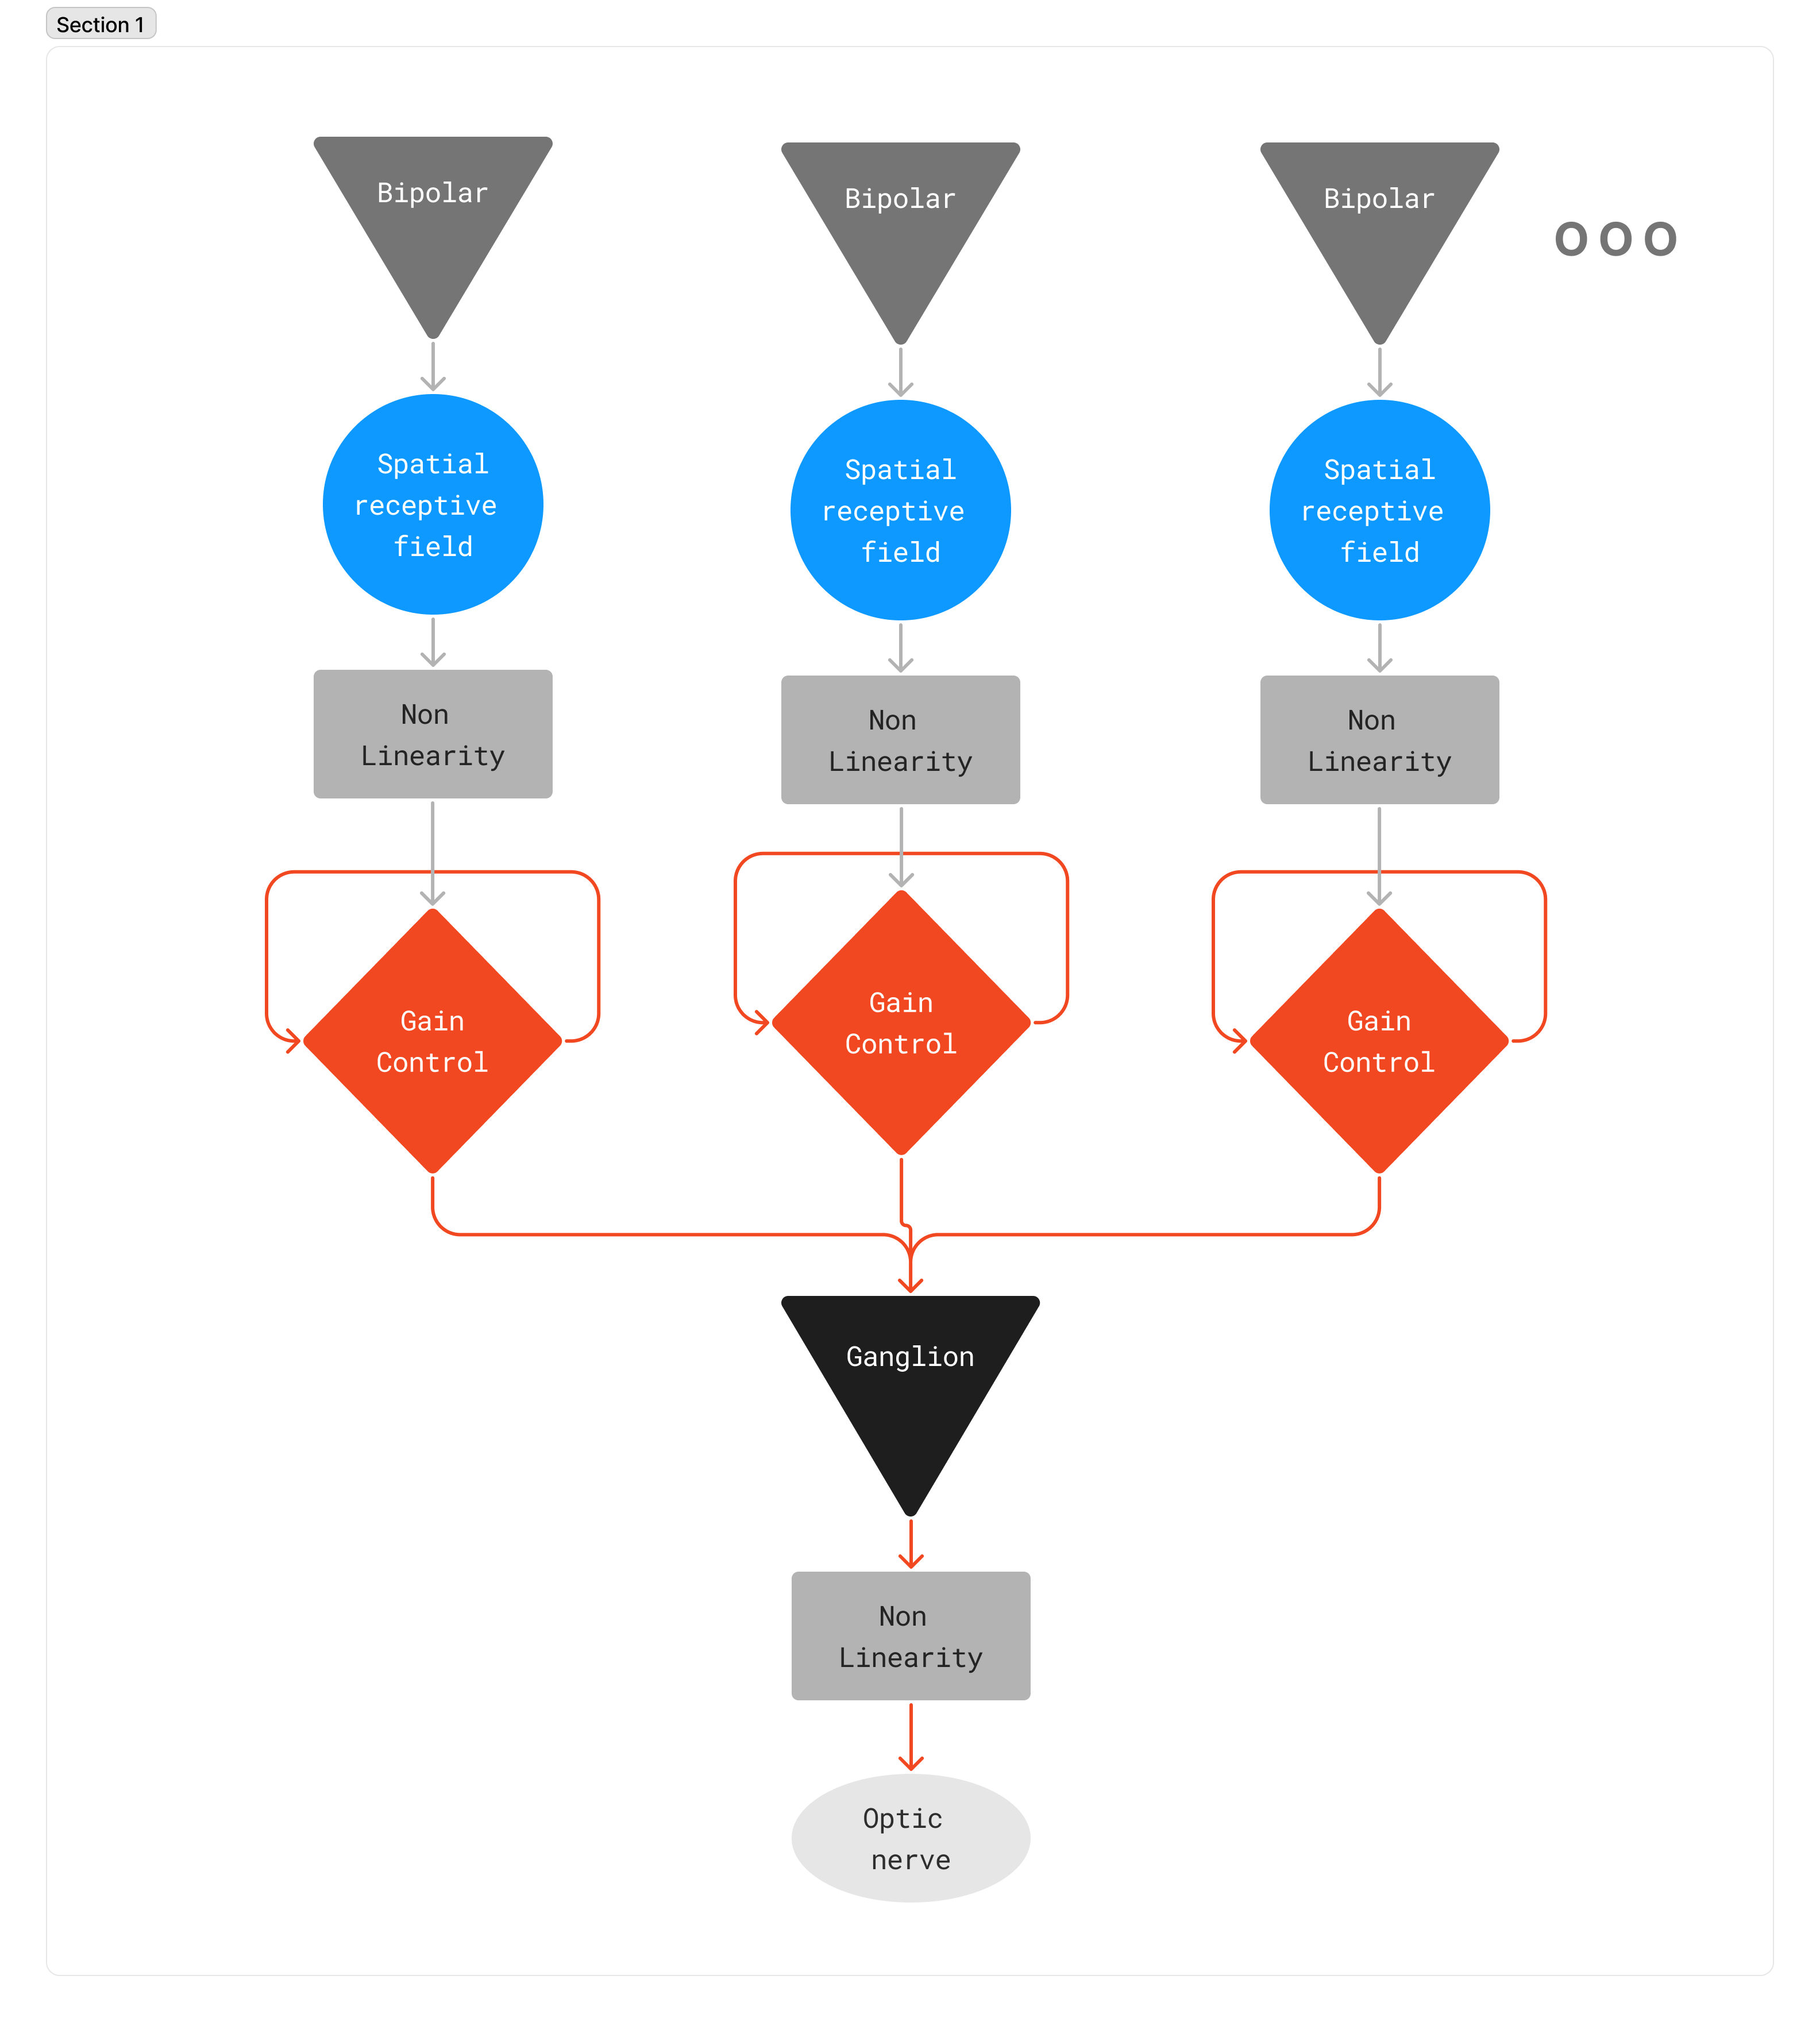
\includegraphics[width=0.95\textwidth]{pics/GCModelDiagram.png}
        \label{fig:LNLN}
    \end{subfigure}%
    \begin{subfigure}{.5\textwidth}
        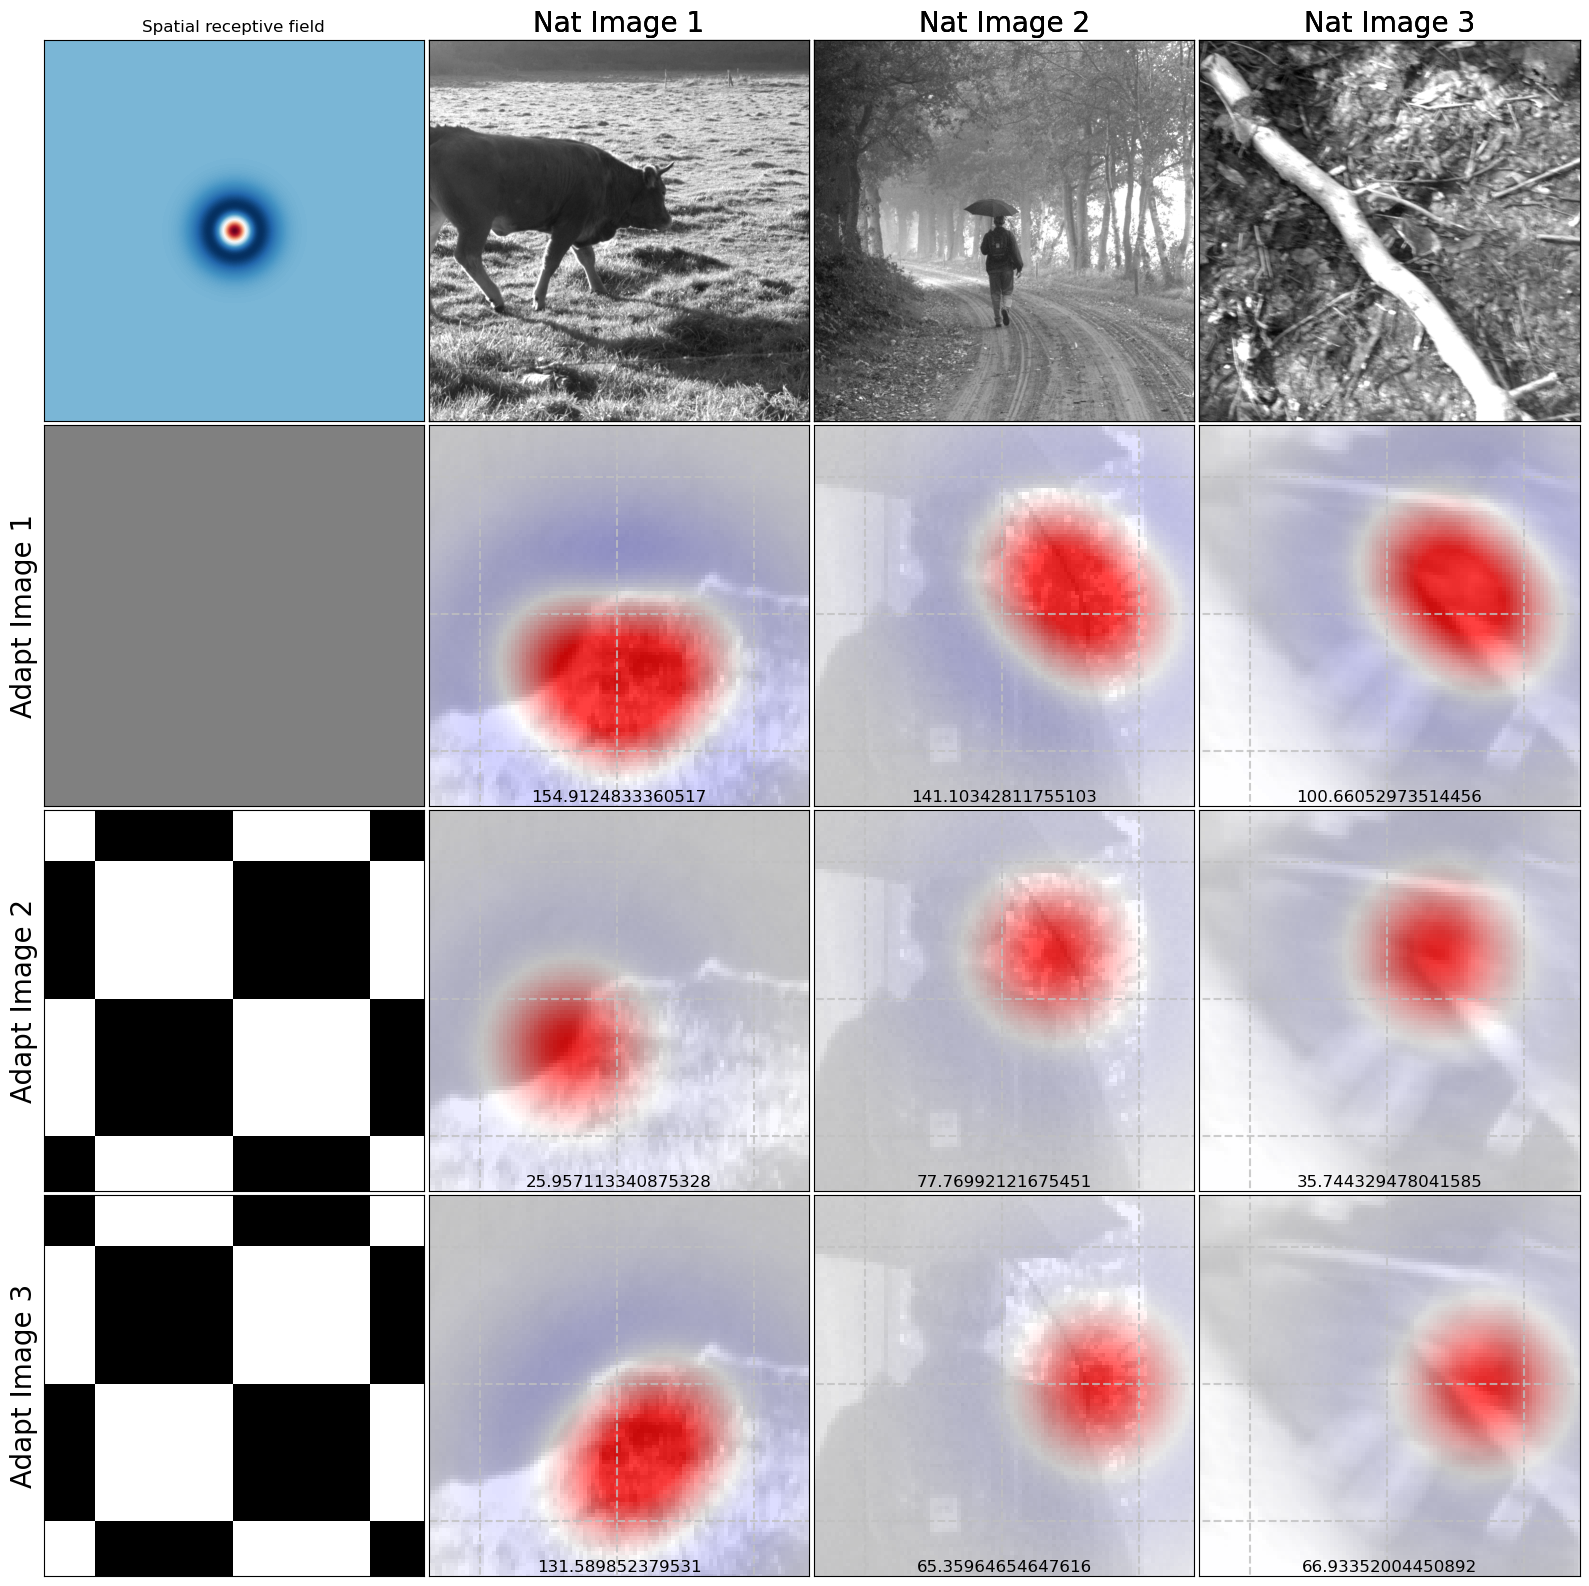
\includegraphics[width=0.95\textwidth]{pics/exModel.png}
        \label{fig:ToyModel}
    \end{subfigure}
    \caption{\textbf{Left: Quick sketch of a gain control LNLN model.} Each
        bipolar
        cell is
        composed of a linear spatial filter that selectively responds to part
        of the scene,
        a non-linear activation function, and a gain control mechanism that
        scale its output
        depending on past events. They all converge into one bipolar cell
        (forming its receptive field)
        of which output is also modeled using a non-linear function.
        textbf{Right.} Recreating displacement of LSTA with a Gain
        Control toy model.}
\end{figure}

\clearpage